\mainchapter{Methods}{0.55}{After some tedious algebra, that is left as an exercise to the reader\ldots}{E. Landi Degl’Innocenti,\\\textit{Polarization in Spectral Lines}} \label{chap:methods}

%----------------------------------------%
% Methods
%----------------------------------------%

We have performed long-term simulations of CCSNe in one and two dimensions, from \(\sim1\units{s}\) after bounce until shock breakout from the stellar surface, several tens of hours afterwards. To do so at a reasonable computational cost, we have implemented an inner boundary condition designed to mimic the neutrino-driven wind forming around the PNS. This chapter presents the progenitors and the tools used for the simulations as well as the details of the methods employed.

\section{Numerical setup} \label{sec:setup}

In this thesis, we used two progenitors to perform 1D and 2D simulations. The 1D simulations utilised a zero-metallicity, \(M_\mathrm{ZAMS} = 9.6\sunmass\) progenitor star from A. Heger (private communication), and the 2D simulations utilised a solar-metallicity, \(M_\mathrm{ZAMS} = 12\sunmass\) progenitor from \cite{Woosley2007} (thenceforth referred to as the z9.6 and s12 progenitors, respectively). Note that we refer to the Zero-Age Main-Sequence (ZAMS) mass, which corresponds to the mass of the star at its entry on the main sequence. The final mass of the star at moment of collapse is determined by processes such as stellar winds, that have caused it to lose mass during the course of its life, and depends on the stellar evolution models used to produce the progenitor.

The simulations are carried out in two phases. A first simulation is ran from moment of collapse until \(\sim1\text{-}2\units{s}\) after core bounce, and a second, long-term simulation continues until shock breakout from the stellar surface using the inner boundary conditions described in \Cref{sec:bdry_condition} along with simpler physics. 

\subsection{FLASH}

All the simulations presented in this thesis are carried out utilising a modified version of the \flash\ framework (version 4) \citep{Fryxell2000, Dubey2009}. The \flash\ code is a modular, multiphysics, Newtonian hydrodynamics code. It can simulate using spherical coordinates in one dimension, assuming spherical symmetry, with cylindrical coordinates in two dimensions, assuming axisymmetry, and with Cartesian coordinates in three dimensions, assuming no symmetry. \flash\ uses a uniform grid with Adaptive Mesh Refinement (AMR). AMR is a numerical technique used to refine the grid locally in order to obtain a higher resolution where needed, whilst saving computational time in places where a lower resolution is sufficient. Refinement and derefinement is determined by a user-defined error criterion, and the time step is set by the Courant–Friedrichs–Lewy (CFL) condition. In \flash, this condition is written as follows
\begin{equation}
    C = (c_s \pm u) \frac{\Delta t}{\Delta x} \punct{,}
\end{equation}

where \(c_s\) and \(u\) are the local sound speed and flow velocity, \(\Delta t\) is the local time step and \(\Delta x\) is the cell size. The value of the CFL condition \(C\) being known from the configuration of the simulation, \flash\ can solve for the time step using the largest value of \(c_s \pm u\). In \flash, the domain is subdivided in regions called \emph{blocks} that can achieve different levels of refinement. Each additional level of refinement cuts the size of a block in half in each direction, and the block at the highest refinement level is divided in 16 grid cells in every direction. Additionally, \flash\ restricts the jump in refinement from one block to an adjacent one to no more than one level. An example block structure is pictured in \Cref{fig:flash_blocks}.

\begin{figure}[ht!]
    \centering
    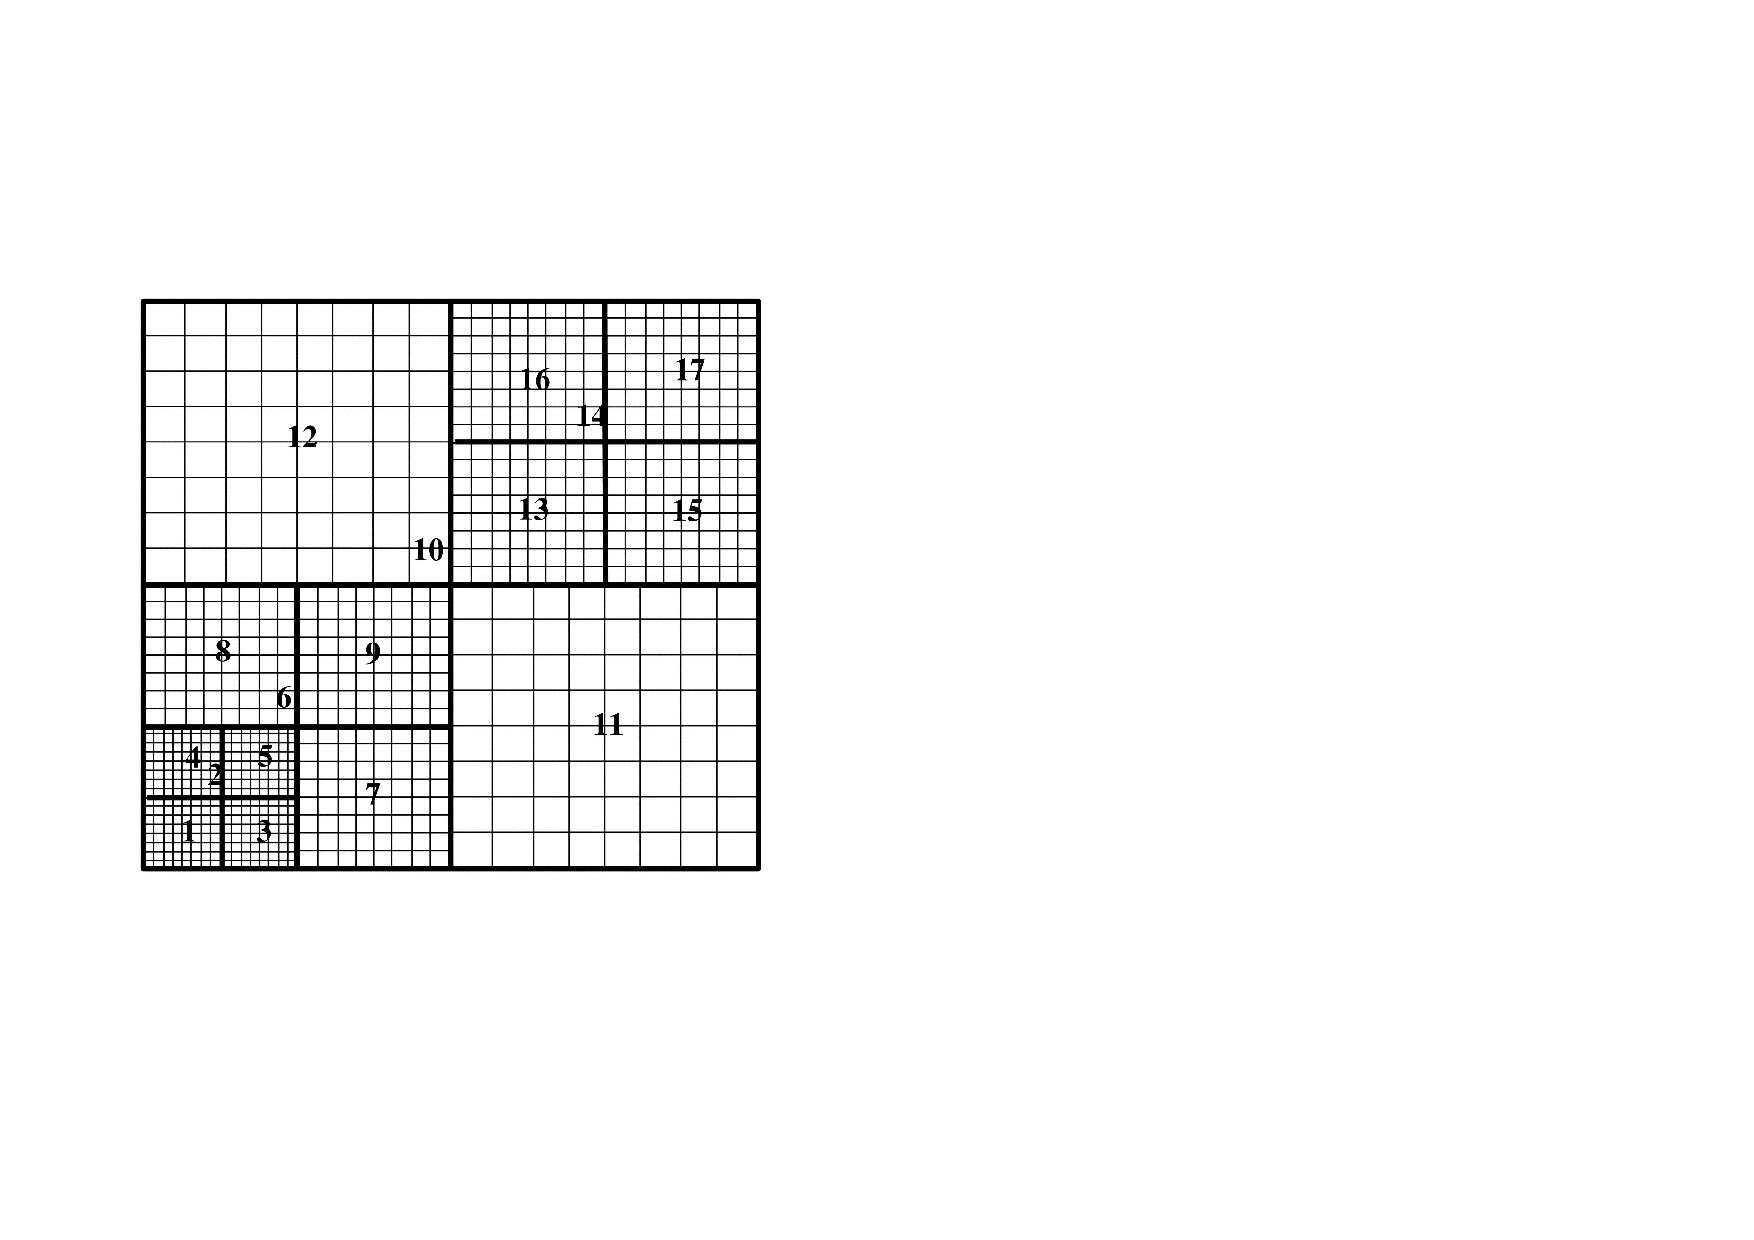
\includegraphics[width=0.55\linewidth]{figures/flash_blocks.pdf}
    \caption{An example set of blocks in \flash. In this example, an interior grid structure of 8x8 cells is also shown, but we use 16x16 for our simulations. The numbers near the centre of the blocks show where the blocks are located in the list of blocks, not shown here. Figure taken from \cite{Fryxell2000}.}
    \label{fig:flash_blocks}
\end{figure}

We use a version of \flash\ specifically adapted for core collapse simulations \citep{Couch2013, Couch2014, OConnor2018a, OConnor2018b}. The code uses a modified general relativistic effective potential to solve gravity (Case A in \citealt{Marek2006}), and evolves three neutrino species using an energy-dependent two-moment neutrino transport scheme with an analytical closure (M1) \citep{OConnor2018a}. This includes electron neutrinos and antineutrinos, as well as a third species collecting all the heavy-lepton neutrinos. Neutrino opacities are generated with the neutrino opacity library NuLib \citep{OConnor2015, Sullivan2016}.

\subsection{Collapse and post-bounce setup} \label{sec:cc_setup}

The z9.6 progenitor is simulated from collapse until \(2.23\units{s}\) after collapse in spherical symmetry (1D) on a domain extending to a radius of \(10^{11}\units{cm}\). Using 16 levels of adaptive mesh refinement, we achieve a finest grid spacing of \(\sim238\units{m}\), with the largest cells being \(\sim7{,}800\units{km}\) across. The energy-dependent neutrino transport is carried out using 12 energy groups. The simulation uses a hybrid EoS, made from a combination of two equations of state. At nuclear densities, such as in the PNS, the SFHo equation of state is used \citep{Steiner2013}, then at lower densities, outside of the PNS, the so-called \emph{Helmholtz EoS} is used instead \citep{Timmes1999}. The latter EoS gives the pressure from the contribution of different species,
\begin{equation}
    P = P_\mathrm{rad} + P_\mathrm{ion} + P_\mathrm{ele} + P_\mathrm{pos}
\end{equation}

where \(P_\mathrm{rad}\), \(P_\mathrm{ion}\),  \(P_\mathrm{ele}\) and  \(P_\mathrm{pos}\) is the radiation pressure, the pressure from the nuclei, and the electron and positron pressures respectively. The different contributions can be computed analytically from the temperature \(T\), the density \(\rho\), the mean number of nucleons per isotope \(\bar{\mathcal{A}}\) and the mean charge per isotope \(\bar{\mathcal{Z}}\), following \cite{Timmes1999}.

The s12 progenitor is simulated from collapse until \(\sim1.2\units{s}\) after collapse in cylindrical coordinates using axisymmetry on the polar axis (2D). The domain extends to a radius of \(6.4 \cdot 10^9\units{cm}\) and covers \(\pm 6.4 \cdot 10^9\units{cm}\) along the polar axis. The simulation uses 11 levels of refinement to obtain a minimum grid spacing of \(\sim488 \units{m}\) in the PNS and maintains an angular resolution of \(0.6\degree\). The simulation uses the same parametrisation for the neutrino transport as for the z9.6 as well as the same EoS. This progenitor has been simulated three times with different heating factors \(f_\mathrm{heat}\) of \(1.0\), \(1.5\) and \(2.0\), i.e a heating factor of \(2.0\) will result in twice as much energy deposited by neutrinos in the gain layer as it should normally do. 
This was done in order to obtain different explosion energies and observe the impact on the explosion mechanism and the evolution of the shock wave.
For simplicity, we henceforth refer to this set of simulations, before time of mapping, as the \emph{initial simulations}.

\subsection{Long-term setup} \label{sec:lt_setup}

To save computational time, the initial simulations are performed only on the most central part of the progenitors for a sufficiently short duration that the shock wave stays far from the boundaries of the domain and that the outer envelope can be assumed to be in equilibrium. Thus, in order to continue the simulation until shock breakout, we must first map the final state of the first simulation, at time of mapping \(t_\mathrm{map}\), to a larger domain that contains the entire star. Because the progenitor models are given in the form of 1D profiles, extending the domain for the 1D simulation is straightforward. The mapping procedure is a little more complex in 2D, but is in essence very similar: we map the result of the initial simulation at time of mapping onto the original progenitor model in order to include the outer parts of the progenitor to the computational domain. More details on the mapping procedure are given in \Cref{sec:mapping}

The long-term simulations are carried out in two steps. First using the outflow boundary condition, described in \Cref{sec:bdry_out}, until the diagnostic explosion energy saturates, which corresponds to approximately the Kelvin-Helmholtz cooling timescale of \(\sim 10\units{s}\). Afterwards, we use the inflow boundary condition, described in \Cref{sec:bdry_in}, for the rest of the simulation until shock breakout. Consequently, the neutrino transport is turned off for these simulations, and the need for a high-density equation of state is eliminated, as the PNS is cut from the domain and replaced by the inner boundary condition. Therefore, only the Helmholtz EoS is used, and a lower resolution of the computational grid is sufficient.  To prevent ambiguities, it should be noted that it is common to refer to the terms \emph{inflow} and \emph{outflow} in the sense of matter flowing in or out of the domain. In this thesis, however, we will refer to \emph{inflow} and \emph{outflow} in the opposite way, as matter flowing towards or away from the PNS.

The long-term simulation of the z9.6 progenitor is ran from \(t_\mathrm{map} = 1.6\units{s}\) after collapse until shock breakout. The new domain extends to \(1.49 \cdot 10^{13}\units{cm}\) and uses 18 levels of refinement, giving a minimum grid spacing of \(\sim8.9\units{km}\).

The long-term 2D simulations of the s12 progenitor are ran from \(t_\mathrm{map} = 1.15\units{s}\) after collapse until shock breakout, the new domain extending to a radius of \(5.24 \cdot 10^{13}\units{cm}\) and covering \(\pm 5.24 \cdot 10^{13}\units{cm}\) along the polar axis. It uses 20 levels of refinement and maintains an angular resolution of \(0.6\degree\), giving a minimum grid spacing of \(\sim7.8\units{km}\).

For all the simulations, the outflow boundary condition is fixed at a radius of \(500\units{km}\). The conditions at the inner boundary are taken from the initial simulations at time of mapping. For the 1D simulation, this is simply the values of the density, internal energy and velocity at \(500\units{km}\). The conditions for the 2D simulations are obtained by spherically averaging the relevant quantities. Unfortunately, for most of the simulations, this gives rather unrealistic values of the velocity, either very low, extremely high, or negative. Thus, most of the 2D simulations were ran with different wind velocities, and the influence of this choice is explored in \Cref{chap:results}. An overview of the long-term simulations and their parametrisation is shown in \Cref{tab:sim_params}, where the different simulations have been labelled based on a combination of the progenitor name, and optionally the heating factor and neutrino wind velocity, in this order.

\begin{table}[ht!]
\begin{threeparttable}[t]
    \caption{Overview of the long-term simulations.}
    \label{tab:sim_params}
    \centering
    \setstretch{1.2}
    \begin{tabular*}{\columnwidth}{@{\extracolsep{\stretch{1}}}*{8}{c}@{}}
    \hline
    \hline
    Name            & Progenitor & \(f_\mathrm{heat}\) & \(t_\mathrm{map}\)\tnote{a} & \(t_\mathrm{hole}\)\tnote{b} & \(v_\mathrm{wind}\) & \(\gamma_{\rho}\) & \(\gamma_{e}\) \\ 
                    &            &                     & [s]                         & [s]                          & [km/s]              &                   &                \\ \hline
    z96             & z9.6       & 1.0                 & 1.6                         & 30.0                         & \(11{,}357\)          & 1.8               & 0.06           \\
    s12hf1p0\_w10e8 & s12        & 1.0                 & 1.15                        & 8.0                          & \(10{,}000\)          & 1.8               & 0.6            \\
    s12hf1p0\_w28e8 & s12        & 1.0                 & 1.15                        & 8.0                          & \(28{,}000\)          & 1.8               & 0.6            \\
    s12hf1p5\_w13e8 & s12        & 1.5                 & 1.15                        & 10.0                         & \(13{,}000\)          & 1.8               & 0.6            \\
    s12hf1p5\_w15e8 & s12        & 1.5                 & 1.15                        & 10.0                         & \(15{,}000\)          & 1.8               & 0.6            \\
    s12hf2p0        & s12        & 2.0                 & 1.15                        & 10.0                         & \(15{,}600\)          & 1.8               & 0.6            \\
    \hline
    \end{tabular*}
    \setstretch{1.0}
    \begin{tablenotes}
        \item[a] Time of mapping from collapse.
        \item[b] Time of change to inflow boundary condition from collapse.
    \end{tablenotes}
\end{threeparttable}
\end{table}

\section{Inner boundary conditions} \label{sec:bdry_condition}

Performing long-term simulations of CCSNe from first principles, including an accurate neutrino transport scheme, a nuclear EoS, and doing so on a domain containing the entire star whilst keeping the necessary resolution inside the PNS, would be too computationally expensive, especially in multiple dimensions. However, we see that these limitations are primarily associated with the PNS and its surroundings. The neutrinos are emitted from the PNS, and their interactions mostly affect the high-density regions in its vicinity, the rest of the star being transparent to them; the nuclear EoS is only needed to describe matter inside the PNS, and the high resolution requirement is due to the relativistic speed of sound in this central part. As was discussed in \Cref{sec:ndw}, about \(1\units{s}\) after collapse, the shock has been revived and has propagated to radii of a few thousand kilometres, while the PNS cools on the Kelvin-Helmholtz timescale. If we wish to look at the long-term evolution of the shock and of the star, we can approximate this cooling phase by a semi-analytical neutrino-driven wind solution around the PNS, thus removing the central part from the simulation and replacing it with an inner boundary condition mimicking this effect. Additionally, we place a point mass at the coordinate origin to account for the monopole contribution to gravity from the PNS and all the material excised from the domain within the inner boundary. This method drastically relaxes the time step constraints imposed by the CFL condition at the centre of the domain. The effect of neutrinos is modelled by the ejecta produced by the neutrino wind, and the need for a nuclear EoS is eliminated.

Following this idea, the long-term simulations are executed in two steps. First, after mapping the final state of the initial simulation onto a larger computational grid, we restart the simulation with an outflow boundary condition at a fixed radius emulating the neutrino wind, similar to that used by \cite{Wongwathanarat2015} and \cite{Stockinger2020}, and do so for approximately the Kelvin-Helmholtz timescale of \(\sim10\units{s}\), until the diagnostic explosion energy saturates. After that, we assume that the neutrino wind has little impact on the rest of the evolution, and replace it with an inflow boundary condition that we let expand for the rest of the simulation, further relaxing the CFL condition.

\subsection{Outflow condition: neutrino wind} \label{sec:bdry_out}

The outflow boundary condition, producing the neutrino wind, is modelled following \cite{Wongwathanarat2015}. The boundary condition is set at a fixed radius, where we impose a constant wind velocity \(v_\mathrm{wind}\), leading to a power-law wind, where two time-dependent quantities, namely the density and internal energy, are evolved as follows:
\begin{gather}
    \rho_\mathrm{wind} = \rho_\mathrm{map} \left( \frac{t}{t_\mathrm{map}} \right)^{-\gamma_\rho} \label{eq:rho_wind} \punct{,} \\
    e_\mathrm{int,wind} = e_\mathrm{int,map} \left( \frac{t}{t_\mathrm{map}} \right)^{-\gamma_e} \label{eq:eint_wind} \punct{.}
\end{gather}

The quantities \(\rho_\mathrm{map}\) and \(e_\mathrm{int,map}\) are the values of the density and internal energy at the inner boundary at time of mapping \(t_\mathrm{map}\), obtained from the profile of the initial simulation. The power-law indices \(\gamma_\rho\) and \(\gamma_e\) are obtained by fitting the time evolution of the density and internal energy at the inner boundary from the initial simulation. The fitting is done using a non-linear least-square approach, where the chi-square statistic is defined as
\begin{equation}
    \chi^2 = \int_{t_\mathrm{map}}^{t_\mathrm{end}} \left[ Q_\mathrm{data}(t) - Q_\mathrm{model}(t, \gamma) \right]^2 \upd[t] \punct{,} \label{eq:chi_square}
\end{equation}

where \(Q_\mathrm{data}(t)\) and \(Q_\mathrm{model}(t, \gamma)\) are the quantities we are fitting (here, either the density or the internal energy) at time \(t\) obtained from the simulation and from the model, respectively. The upper bound of this integral, \(t_\mathrm{end}\), corresponds to the end time of the initial simulation, that was run for a few more \(10\text{-}100\units{ms}\) after time of mapping, depending on the simulation. The best fit corresponds to the fit that minimises the value of \(\chi^2\) for a given model variable \(\gamma\), which here corresponds to our power-law index. The integral in \Cref{eq:chi_square} is admittedly discretised, as the simulation only saves the data at discrete time steps. \Cref{fig:fit_1d} shows the result of the fitting for the 1D simulation. For the 2D simulations, we cannot choose an arbitrary one-dimensional profile from the domain, and a profile obtained from spherically averaging the domain gives very noisy results. Consequently, we have decided to pick the power-law index for the density evolution, \(\gamma_\rho\), from the result of the fitting from the 1D simulation. As for the power-law index for the time evolution of the internal energy, \(\gamma_e\), it is set to \(\gamma_\rho / 3\), following \cite{Wongwathanarat2015}.

\begin{figure}[ht!]
    \centering
    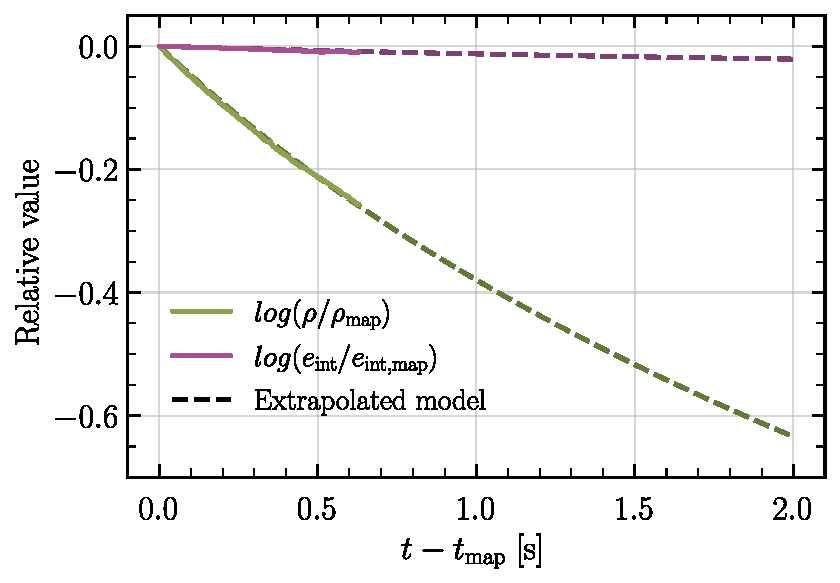
\includegraphics[width=0.75\linewidth]{figures/fit.pdf}
    \caption{Time-dependent behaviour of the neutrino-driven wind density \(\rho\), and internal energy \(e_\mathrm{int}\), from time of mapping \(t_\mathrm{map}\) at \(500\units{km}\), normalised to their mapping values, obtained from the initial 1D simulation of the z9.6 progenitor (solid lines) and extrapolated to later times using the best-fit power-law indices (dashed lines).}
    \label{fig:fit_1d}
\end{figure}

The composition of the ejecta is described by the two quantities \(\bar{\mathcal{A}}\) and \(\bar{\mathcal{Z}} = \bar{\mathcal{A}}Y_e\), and is fixed to represent a composition equivalent to that of alpha particles, therefore \(\bar{\mathcal{A}} = 4\) and \(\bar{\mathcal{Z}} = 2\). This is a somewhat average value, and does not impact considerably our simulations. However, if we were interested in the nucleosynthesis and the actual composition of the neutrino-heated ejecta, we would do so using a nuclear network, and would need to use appropriate values of \(\bar{\mathcal{A}}\), \(\bar{\mathcal{Z}}\) and \(Y_e\).

\subsection{Inflow condition: black hole} \label{sec:bdry_in}

What is referred to as the \emph{diagnostic explosion energy} is defined as the integral of the total energy density (i.e. kinetic, internal and gravitational) in the post-shock region, over volume elements where this quantity is positive. In other words, it is the energy contained in all the material that is unbound from the star. If the neutrino wind is strong enough, we expect an injection of energy to the explosion, as material is accelerated outwards by the wind and escapes the gravitational pull of the neutron star. After a few tens of seconds, once the wind has weakened, due to the drop in density and internal energy, the explosion energy saturates. At this point, we assume the neutrino wind to have little impact on the overall evolution of the explosion. Therefore, the outflow boundary condition is replaced with an inflow boundary condition. This new boundary condition effectively acts like a black hole, although it does not physically correspond to one, in which material falls but is not ejected. This condition is initially set at time \(t_\mathrm{hole}\), and at the same radius as the outflow condition, but expands at a velocity of \(100\units{km/s}\), further relaxing the time step as the boundary goes to larger and larger radii. The shock wave has already evolved very far from the core, and the ejected material has been accelerated to much higher velocities, so that the expansion of the boundary in no way affects the explosion energy.

\section{Implementation details}

To conclude this chapter, we give in this section some additional details on the usage of the \flash\ code, the implementation and internal behaviour of the inner boundary conditions, as well as some other considerations that we must have in order to run the simulations.

\subsection{Mapping procedure} \label{sec:mapping}

The progenitor models are provided in the form of 1D profiles, extending from the centre of the star to its surface, and give values of essential quantities (density, temperature, pressure, velocity, electron fraction, etc.) at different radii. When initialising a simulation, \flash\ reads the content of this model, creates a grid covering all radii, and fills each cells with values interpolated from the 1D profile. It is then possible to initialise a simulation on a reduced domain, only containing the central part of the star, by excluding the outer part of the progenitor's profile, as is done in the case of the initial simulations. When we wish to reintroduce the outer region to perform long-term simulations, we do so in 1D by simply appending this region of the progenitor's profile to the evolved profile of the simulation, and restarting \flash\ using the resulting, extended profile. \flash\ is then capable of determining the values of \(\rho_\mathrm{map}\), \(e_\mathrm{int,map}\) and \(v_\mathrm{wind}\) by evaluating the profile at the inner boundary, i.e \(500\units{km}\). In 2D, this procedure is more complex. We start by creating a 1D profile from a spherical average of the evolved, initial simulation to which we append the outer region of the progenitor's profile, such as in the 1D case. We then let \flash\ initialise a new 2D grid for the long-term simulation using the resulting profile, but without evolving it. It normally extracts values for the density, internal energy, and velocity for the neutrino wind from this spherically averaged profile, and initialises the inner boundary condition on the new 2D grid. This new grid now contains the outer region of the progenitor with the initialised inner boundary corresponding to the neutrino wind, but a spherical average of the initial simulation in the middle region. Using an external tool pipeline, we then remap the evolved 2D grid of the reduced domain from the initial simulation onto the new 2D grid, excluding the inner region that now contains the neutrino wind. The result is a 2D grid of the complete domain, containing the neutrino wind at its centre, the evolved region from the initial simulation at \(t_\mathrm{map}\), and the outer part of the progenitor, that can now be evolved to late times using \flash.

\subsection{Inner boundary structure} \label{sec:bdry_structure}

In principle, we want our boundary condition to be modelled as the surface of a region excised from the simulation, on which we prescribe values for the density, internal energy and velocity, constraining the hydrodynamical evolution of the adjacent cells. However, our version of \flash\ does not model our inner boundary condition in this way. Because \flash\ uses a Cartesian grid in 2D and 3D, our spherical inner boundary is not a smooth surface, but rather resembles a \emph{voxelised} structure made of square cells, not very suitable for such a description of a boundary condition. But more importantly, this would violate conservation, as mass and energy would be created and injected in the simulation from this surface. Consequently, the cells within the region inside the inner boundary, that we commonly refer to as \emph{the hole}, are still evolved normally, but \flash\ calls a routine after each time step that lets us adjust the conditions within these cells to match the desired state of our inner boundary. As a remark, the conditions inside the hole are still much more gentle than in the PNS, and this is sufficient to drastically reduce the resolution required in this region, so that the cost of evolving these inner cells is almost negligible. Any deviation from the expected mass in the cells within the inner region is then corrected using the mass contained in the point mass, and therefore preserves conservation in the system. Moreover, this means that mass can still accrete onto the boundary. The accreted mass would then be added to the point mass, and it becomes possible to follow the evolution of accretion on the central region at late times.

We note however that, because the cells in the inner region are still evolved, for the inner boundary condition to have the expected influence on the outside region, we must ensure that pressure support is kept inside the boundary. We do this by prescribing a power-law radial profile to the density and internal energy in order to have approximate hydrostatic equilibrium inside the hole. This is further discussed in \Cref{chap:results}.

\subsection{Point mass correction} \label{sec:pm_correction}

The \flash\ code is a Newtonian hydrodynamics code, which implies that the baryonic mass in the system is conserved during the simulation, but the neutrinos take out a non-negligible fraction of the total energy of the PNS, reducing the gravitational mass. This is taken in account in the code during the calculation of the effective gravitational potential mentioned earlier (Case A of \citealt{Marek2006}). However, this is not possible after mapping as we have placed all the mass, including the PNS, within the inner boundary inside a point mass. Thus, we must add a correction to the point mass at time of mapping to account for the loss of gravitational mass from the neutrino emission. This correction is calculated using the following expression:
\begin{equation}
    \Delta M = \frac{1}{c^2} \int_0^{t_\mathrm{map}} \left( L_{\nu_e} + L_{\bar{\nu_e}} + 4 L_{x} \right) \upd[t] \punct{,}
\end{equation}

where \(c\) is the speed of light, \(L_{\nu_e}\) and \(L_{\bar{\nu_e}}\) are the electron neutrino and antineutrino luminosities, and \(L_{x}\) is the heavy-lepton neutrino luminosity, which is multiplied by four, for each flavour of heavy-lepton neutrino (i.e. \(\mu\) and \(\tau\) neutrinos and antineutrinos). The value of this correction is given in \Cref{tab:pm_correction} for each simulation, and subtracted from the point mass at time of mapping.

\begin{table}[ht!]
\begin{threeparttable}
    \caption{Point-mass corrections for each simulation.}
    \label{tab:pm_correction}
    \centering
    \setstretch{1.2}
    \begin{tabular*}{\columnwidth}{c|@{\extracolsep{\stretch{1}}}*{4}{c}@{}}
         \hline
         \hline
         Simulation & z96 & s12hf1p0 & s12hf1p5 & s12hf2p0 \\
         Point mass correction [g] & \(1.032 \cdot 10^{32}\) & \(1.363 \cdot 10^{32}\) & \(1.226 \cdot 10^{32}\) & \(1.169 \cdot 10^{32}\) \\ \hline
    \end{tabular*}
\end{threeparttable}
\end{table}
